\documentclass{scrartcl}

\usepackage{german}
\usepackage[utf8]{inputenc}  %Umlaute
\usepackage[T1]{fontenc}     %Umlauttrennung
\usepackage{lmodern}         %modernes Schriftbild
\usepackage{amsmath}         %math Umgebungen
\usepackage{graphicx}
\usepackage{hyperref}        %URLs
\usepackage{gensymb}         %Gradzeichen
\usepackage{float}           %Positionierung von Tabellen und Abb
\usepackage{textgreek}


\begin{document}
\begin{titlepage}
  \begin{center}
    \vspace*{1cm}
    \LARGE
    Physikpraktikum für Naturwissenschaftler \\
    \vspace*{1cm}
    \Huge
    \textbf{Versuch: Wechselstromkreise} \\
    \vspace*{0.3cm}
    \Large
    Durchgeführt am 10. Januar 2019 \\
    Betreuer: David Reinhardt \\
    \vspace*{2.5cm}
    Gruppe 13 \\
    Felix Burr: felix.burr@uni-ulm.de \\
    Johannes Spindler: johannes.spindler@uni-ulm.de \\
    \vfill 
  \end{center}
  Wir bestätigen hiermit, das Protokoll selbstständig erarbeitet zu haben und in genauer Kenntnis über dessen Inhalt zu sein. \\
  \vspace*{0.8cm}
  \\
  Felix Burr
  \hfill
  Johannes Spindler
\end{titlepage}
\pagebreak
\tableofcontents


\pagebreak

\section{Einleitung}
Aus dem Ohm'schen Gesetz ist der elektrische Widerstand $R$ als konstantes Verhältnis der Spannung $U$ zur Stromstärke $I$ bekannt:
\begin{align}
R = \frac{U(t)}{I(t)} = const
\end{align}
Das gilt für Gleich- wie Wechselspannungen, allerdings spricht man bei Wechselstromkreisen vom Scheinwiderstand $|Z|$, der als Betrag der (komplexwertigen) Impedanz $Z$ definiert ist:
\begin{align}
|Z| = \frac{U_{0}}{I_{0}}
\end{align}
$U_{0}$ und $I_{0}$ bezeichnen die Amplitudenwerte von Spannung und Stromstärke.

Die Impedanz eines Zweipols fasst im Realteil den Wirkwiderstand $R$ und im Imaginärteil den Blindwiderstand $X$ zusammen. Während beim Wirkwiderstand die Sinuskurven von Spannung und Strom phasengleich sind, liegt beim Blindwiderstand eine Phasenverschiebung von +90\degree oder -90\degree vor. Diese Phasenverschiebung ist der Grund, warum Wirk- und Blindwiderstände einer Schaltung nicht einfach zu einem Gesamtwiderstand addiert werden dürfen, sondern als komplexwertige Impedanz $Z$ verstanden werden. 

\begin{align}
Z = R + iX
\end{align}
Vektoriell betrachtet ist $Z$ ein Vektor mit einer $R$-Komponente auf der x-Achse und einer $X$-Komponente auf der y-Achse. Dann ist der Winkel $\varphi$ zwischen x-Achse und $Z$ der Phasenwinkel und die Länge $|Z|$ des Vektors der Scheinwiderstand.

Im ersten Versuch wird der Scheinwiderstand $|Z|$ für einen Widerstand, einen Kondensator und eine Spule bestimmt. Im zweiten Versuch sollen Impedanz und Phasenverschiebung eines unbekannten Zweipols bestimmt und der Aufbau dieses Zweipols durch Vergleich mit Theoriewerten gefolgert werden.
\section{Impedanzmessung an Widerstand, Kondensator und Spule}
\subsection{Versuchsaufbau und Durchführung}
Es werden vier Messungen durchgeführt: ein Widerstand, ein Kondensator und eine Spule werden mit dem Analog-Oszilloskop vermessen, anschließend die Spule nochmals mit einem Digital-Oszilloskop.

Der zu messende Zweipol wird wie in Abbildung \ref{fig:Aufbau} mit einem bekannten Widerstand $R_{I}$, der zur Bestimmung von $I$ dient, in Reihe geschaltet und an einen Frequenzgenerator und ein Oszilloskop angeschlossen. Abbildung \ref{fig:Aufbau_Foto} zeigt den Aufbau. Als Frequenz wird für Widerstand und Kondensator $f = 1kHz$ und für die Spule $f = 10kHz$ gewählt. Auf Kanal 1 des Oszilloskops wird die Amplitude $U_{1}$ der am Zweipol anliegenden Spannung und auf Kanal 2 die Amplitude $U_{2}$ der an R\textsubscript{I} anliegenden Spannung gemessen. 

\begin{figure}[H]
  \centering
    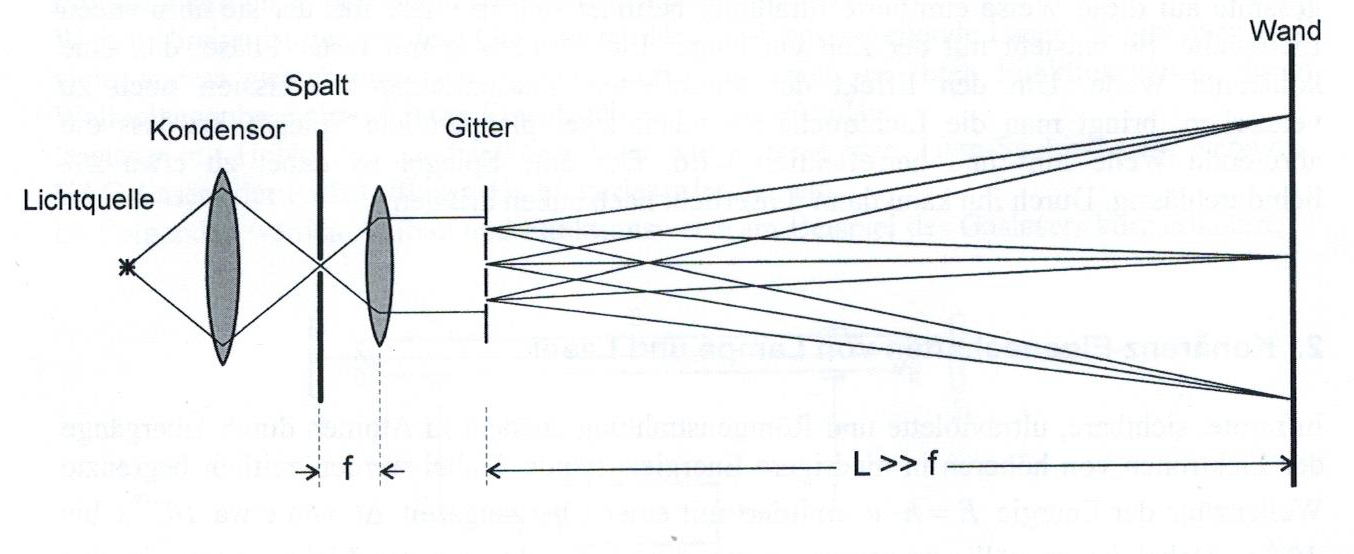
\includegraphics[scale=0.75]{Aufbau.PNG}
  \caption{Schaltbild zur Impedanzmessung (aus der Versuchsanleitung)}
  \label{fig:Aufbau}
\end{figure}

\begin{figure}[H]
  \centering
    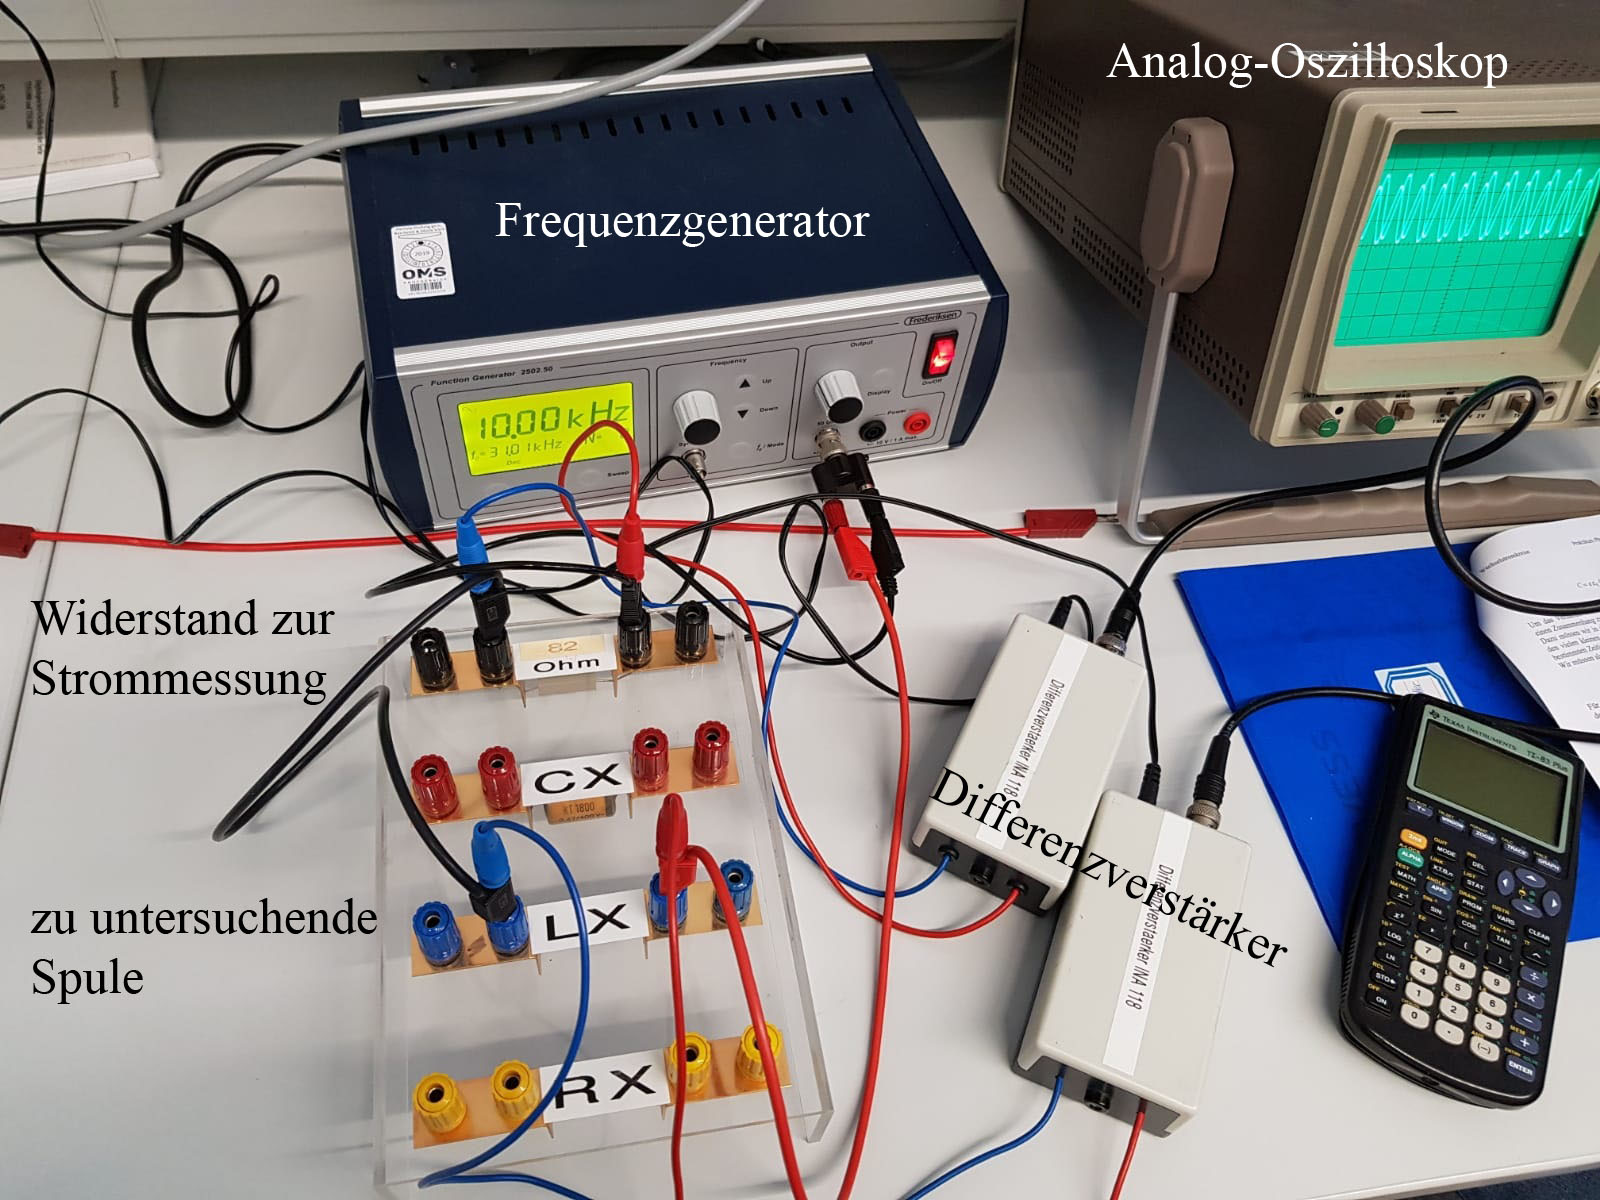
\includegraphics[scale=0.45]{Aufbau_Foto.JPG}
  \caption{Aufbau des Schaltbildes in Abbildung \ref{fig:Aufbau}}
  \label{fig:Aufbau_Foto}
\end{figure}
Mit $U_{2}$ und $R_{I} = 82 \Omega$ kann dann die Stromstärke berechnet werden:
\begin{align}
I = \frac{U_{2}}{R_{I}}
\end{align}
Damit wird der Scheinwiderstand bestimmt:
\begin{align}
|Z| = \frac{U_{1}}{I} = \frac{U_{1}}{U_{2}} \cdot R_{I}
\end{align}

\begin{figure}[H]
  \centering
    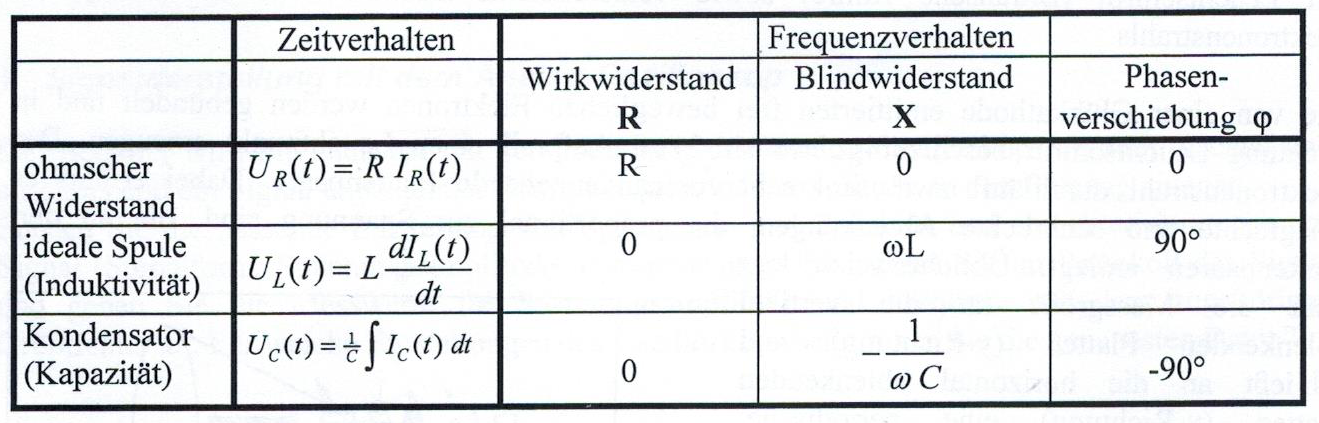
\includegraphics[scale=0.75]{Tabelle.PNG}
  \caption{Zeit- und Frequenzverhalten elementarer Zweipole (aus der Versuchsanleitung)}
  \label{fig:Tabelle}
\end{figure}
Abbildung \ref{fig:Tabelle} zeigt das Zeit- und Frequenzverhalten eines Widerstands, eines Kondensators und einer Spule. Da bei jedem dieser elementaren Zweipole eine Komponente von $Z$ null ist, können die Größen $R$ bzw. $L$ bzw. $C$ leicht aus $|Z|$ berechnet werden:
\begin{align}
R &= |Z| \\
C &= \frac{1}{\omega |Z|} \\
L &= \frac{|Z|}{\omega}
\end{align}
Hierbei ist $\omega = 2 \pi f$ die Kreisfrequenz.

Außerdem soll mit dem Oszilloskop die zeitliche Phasenverschiebung $\Delta t$ zwischen von $U_{1}$ in Bezug auf $U_{2}$ gemessen werden. Daraus kann durch folgendes Verhältnis auch die Phasenverschiebung $\varphi$ in Grad berechnet werden:
\begin{align}
\frac{\varphi}{360\degree} = \frac{\Delta t}{T} = \Delta t \cdot f
\end{align}

\subsection{Messwerte und Ergebnisse}
In Tabelle \ref{tab:Impedanzmessung} wird die für den Zweipol charakteristische Größe $R$/$C$/$L$ und in Tabelle \ref{tab:Phasenmessung} die Phasenverschiebung zwischen Spannung und Strom ermittelt.
\begin{table}[H]
\captionof{table}{Messwerte für $U_{1}$, $U_{2}$ und daraus errechnete Werte für $I$, $|Z|$ und $R$ bzw. $C$ bzw. $L$.}
\begin{center}
\begin{tabular}{l|l|l|l|l|l|l}
Messung    & f [kHz] & U\textsubscript{1} [V] & U\textsubscript{2} [V] & I [A] & |Z| [\textOmega] &  \\
\hline
Widerstand        &  1 & 0,55    & 0,45   & 0,00549   & 100,222    & R = 100,222 \textOmega \\
Kondensator       &  1 & 1,2     & 0,305  & 0,00372   & 322,623    & C = 4,933 $\cdot$ 10\textsuperscript{-7} F \\
Spule             & 10 & 1,2     & 0,26   & 0,00317   & 378,462    & L = 6,023 mH \\
Spule (digital)   & 10 & 1,16    & 0,27   & 0,00329   & 352,296    & L = 5,606 mH
\end{tabular}
\end{center}
\label{tab:Impedanzmessung}
\end{table}

\begin{table}[H]
\captionof{table}{Messwerte für $\Delta t$ und daraus errechnete Werte für $\varphi$.}
\begin{center}
\begin{tabular}{l|l|l|l}
Messung    & f [kHz] & \textDelta t [ms] & \textphi [\degree] \\
\hline
Widerstand        & 1 &  0       & 0       \\
Kondensator       & 1 & -0,22    & -79,2   \\
Spule             & 10 &  0,021   & +75,6   \\
Spule (digital)   & 10 &  0,026   & +93,6   
\end{tabular}
\end{center}
\label{tab:Phasenmessung}
\end{table}

\subsection{Fehlerrechnung}
Die Spannung kann mit einer Genauigkeit von $\Delta U_{1} = \Delta U_{2} = 0,025V$ am Oszilloskop abgelesen werden. Damit ergibt sich für die Größtfehler der Zweipolgrößen:
\begin{align*}
\Delta R &= \Delta |Z| = \left| \frac{\partial R}{\partial U_{1}} \right| \Delta U_{1} + \left| \frac{\partial R_{2}}{\partial U_{2}} \right| \Delta U_{2} = \frac{R_{I}}{U_{2}} \cdot \Delta U_{1} + \frac{R_{I}U_{1}}{U_{2}^2} \cdot \Delta U_{2} = 10,12 \Omega \\
\Delta C &= \left| \frac{\partial C}{\partial |Z|} \right| \Delta |Z| = \frac{1}{\omega |Z|^2} \cdot \Delta |Z| = 5,07 \cdot 10^{-8} F\\
\Delta L &= \left| \frac{\partial L}{\partial |Z|} \right| \Delta |Z| = \frac{1}{\omega} \cdot \Delta |Z| = 7,05 \cdot 10^{-4} H
\end{align*}
\section{Impedanzmessung an einem unbekannten Zweipol}
\subsection{Versuchsaufbau und Durchführung}
In diesem Versuch untersuchen wir einen unbekannten Zweipol, welcher mit einem Ohm'schen Widerstand in Reihe geschaltet wurde. Bei unterschiedlichen Frequenzen messen wir jeweils  die Spannungsdifferenzen an den Widerständen und die zeitliche Phasenverschiebung zwischen den Widerständen.

\begin{figure}[H]
  \centering
    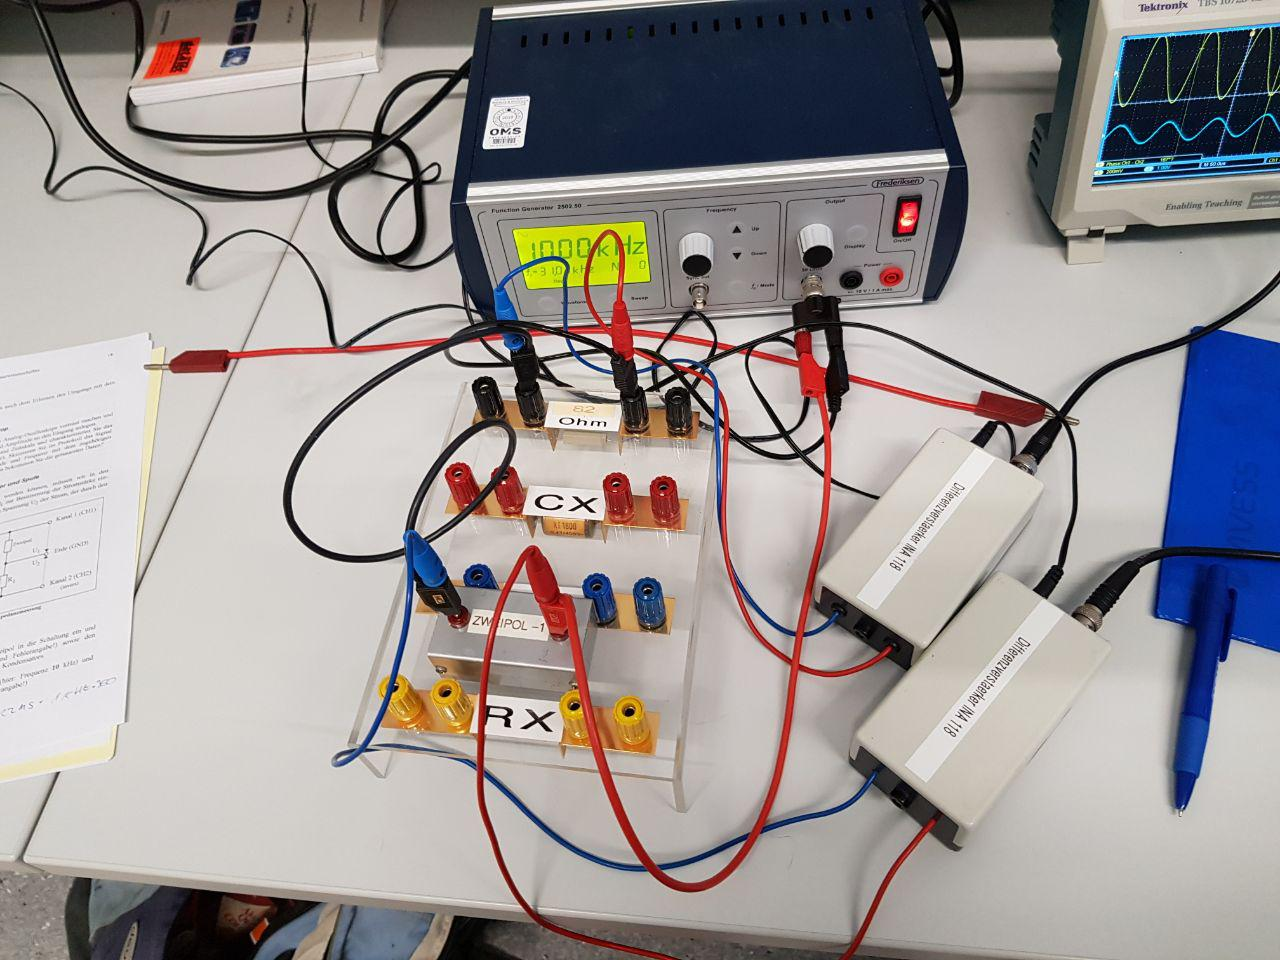
\includegraphics[width=0.75\textwidth]{V_3_Aufbau.jpg}
  \caption{Versuchsaufbau mit unbekannten Zweipol}
  \label{fig:v3a}
\end{figure}
\subsection{Messwerte und Ergebnisse}
\begin{table}[H]
\captionof{table}{Messwerte für $U_1$ und $U_2$ und daraus errechnete Werte}
\begin{center}
\begin{tabular}{l|l|l|l|l|l|l|l}
f [kHz] & $\omega$ [$\frac{rad}{s}$] & $U_1$ [V] & $U_2$ [V] & I [mA] & |Z| [$\Omega$] & $\delta$t [ms] & $\Phi$ [$\degree$]\\ 
\hline
30	&188	&0,01	&1,28&	0,0001219	&10496	&-7,2	&-102,24\\
60	&376	&0,02	&1,32&	0,0002439	&5412	&-4	&-93,6\\
100	&628	&0,0344	&1,32&	0,0004195	&3146	&-2,4	&-93,6\\
200	&1256	&0,068	&1,32&	0,0008292	&1591	&-1,3	&-86,4\\
400	&2513	&0,132	&1,32&	0,001609	&820	&-0,68	&-82,08\\
1000&	6283&	0,272&	1,08&	0,003317&	325	&-0,3	&-72\\
2000&	12566&	0,368&	0,88&	0,004487&	196	&-0,17	&-57,6\\
4000&	25132&	0,44&	0,72&	0,005365&	134	&-0,104	&-30,24\\
10000&	62831&	0,46&	0,65&	0,005609&	115	&-0,046	&-14,4\\
20000&	125663&	0,46&	0,64&	0,005609&	114	&-0,024	&-7,2\\
40000&	2513273&	0,48&	0,62&	0,005853&	105	&-0,0124&	-1,44\\
80000&	502654&	0,48	&0,6	&0,005853	&102,5	&-0,0062&	-1,44\\
\end{tabular}
\end{center}
\label{tab:Phasenmessung}
\end{table}
\begin{figure}[H]
  \centering
    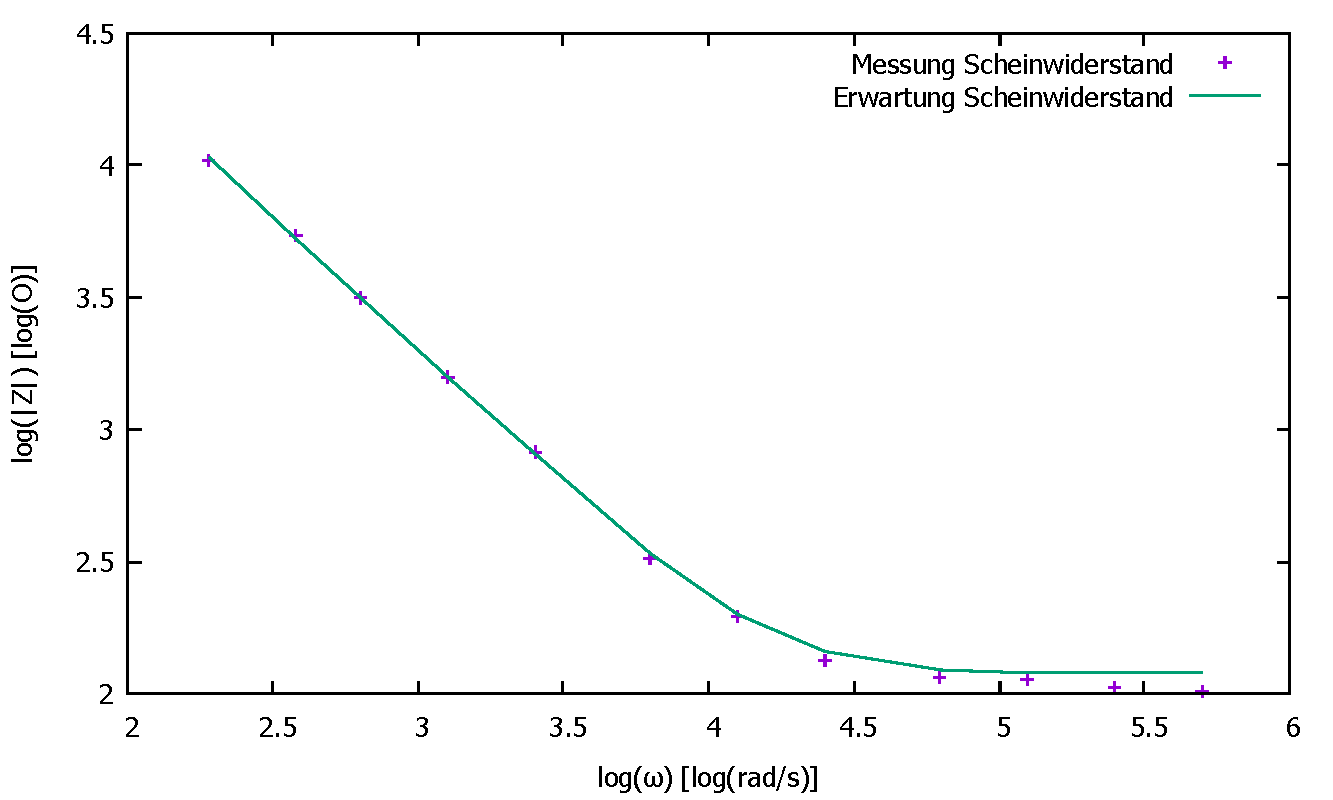
\includegraphics[width=\textwidth]{logo.pdf}
  \caption{Vergleich des gemessenen Scheinwiderstandes zu dem Erwarteten}
  \label{fig:Aufbau_Foto}
\end{figure}
\begin{figure}[H]
  \centering
    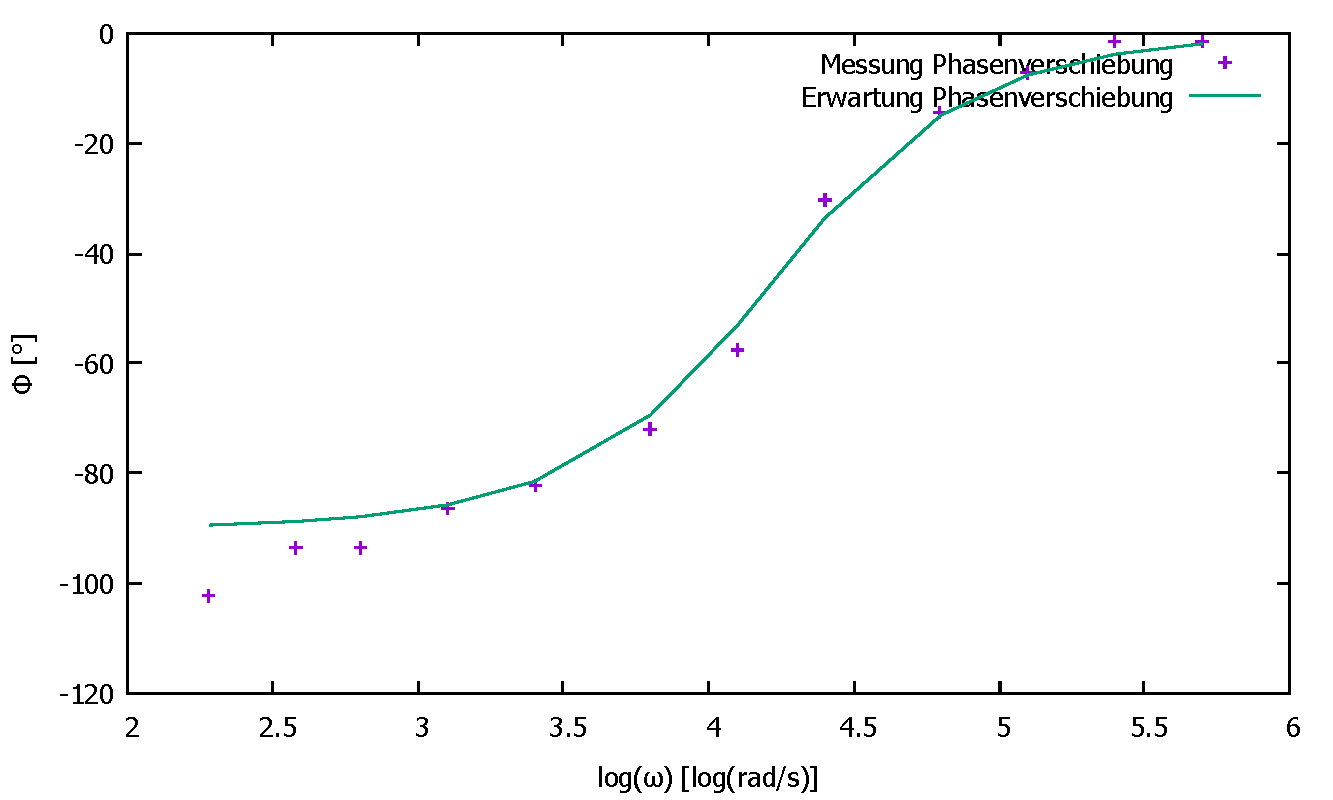
\includegraphics[width=\textwidth]{logo_.pdf}
  \caption{Vergleich der gemessenen Phasenverschiebung zu dem Erwarteten}
  \label{fig:Aufbau_Foto}
\end{figure}
\subsection{Ergebinsdiskussion}
Bei im niederen Frequenzbereich verhält sich der Scheinwiderstand wie eine Spule, und
wir haben eine Phasenverschiebung um $-90\degree$ Im höheren Frequenzbereich verhält sich
der Scheinwiderstand wie ein ohm’scher Widerstand, und die Phasenverschiebung nähert
sich 0 an. Wir schließen daraus, dass eine Kondensator und ein ohm’scher Widerstand in Reihe
geschaltet sind, da sich beide Scheinwiderstände addieren.
Mit kleineren Abweichungen decken sich unsere Messungen gut mit den erwarteten Ergebnissen. Betrachten wir den hohen Frequenzbereich, fällt der Induktive Anteil nicht
ins Gewicht. Für den Ohm’schen Widerstand können wir aus Tabelle 3 $R = 109,125 \pm 5,46$ $\Omega$
als Mittelwert ermitteln. Der Induktive Anteil lässt sich mittels dem Durchschnitt der ersten 6 Messpunkte mittels $C = \frac{1}{\omega * \sqrt{Z^2 - R^2}} = (4,944 \pm 0,163 )*10^{-7}$ $F$ ermitteln

\section{Fazit}
Falls unbekannte Bauteile in einer Schaltung ermittelt werden müssen, ist es nützlich ein
bekanntes Bauteil mit der Schaltung in Reihe zu schalten. So kann man mittels Messungen zwischen den Bauteilen unterscheiden. Der Verlauf der Scheinwiderstandskurve sagt
aus, ob das Bauteil induktive oder kapazitive Elemente enthält. Phasenverschiebungen
geben zusätzlich Aufschluss darüber. Mit den Kirchhoff’schen Regeln und Maschenregeln
lassen sich die anderen Werte ermitteln
\end{document}
